\section{SDSS}
\bartchapterimage{heic0506a_small.jpg}
\bartthumb{thumbs/heic0506a.png}
\subsection{Galaxy sample}
\begin{frame}
    \frametitle{Application to SDSS}
    % \begin{columns}
        % \begin{column}{0.6\linewidth}
            % \begin{minipage}[c][0.7\textheight][c]{\linewidth}
                % \only<-3>{%
                    % 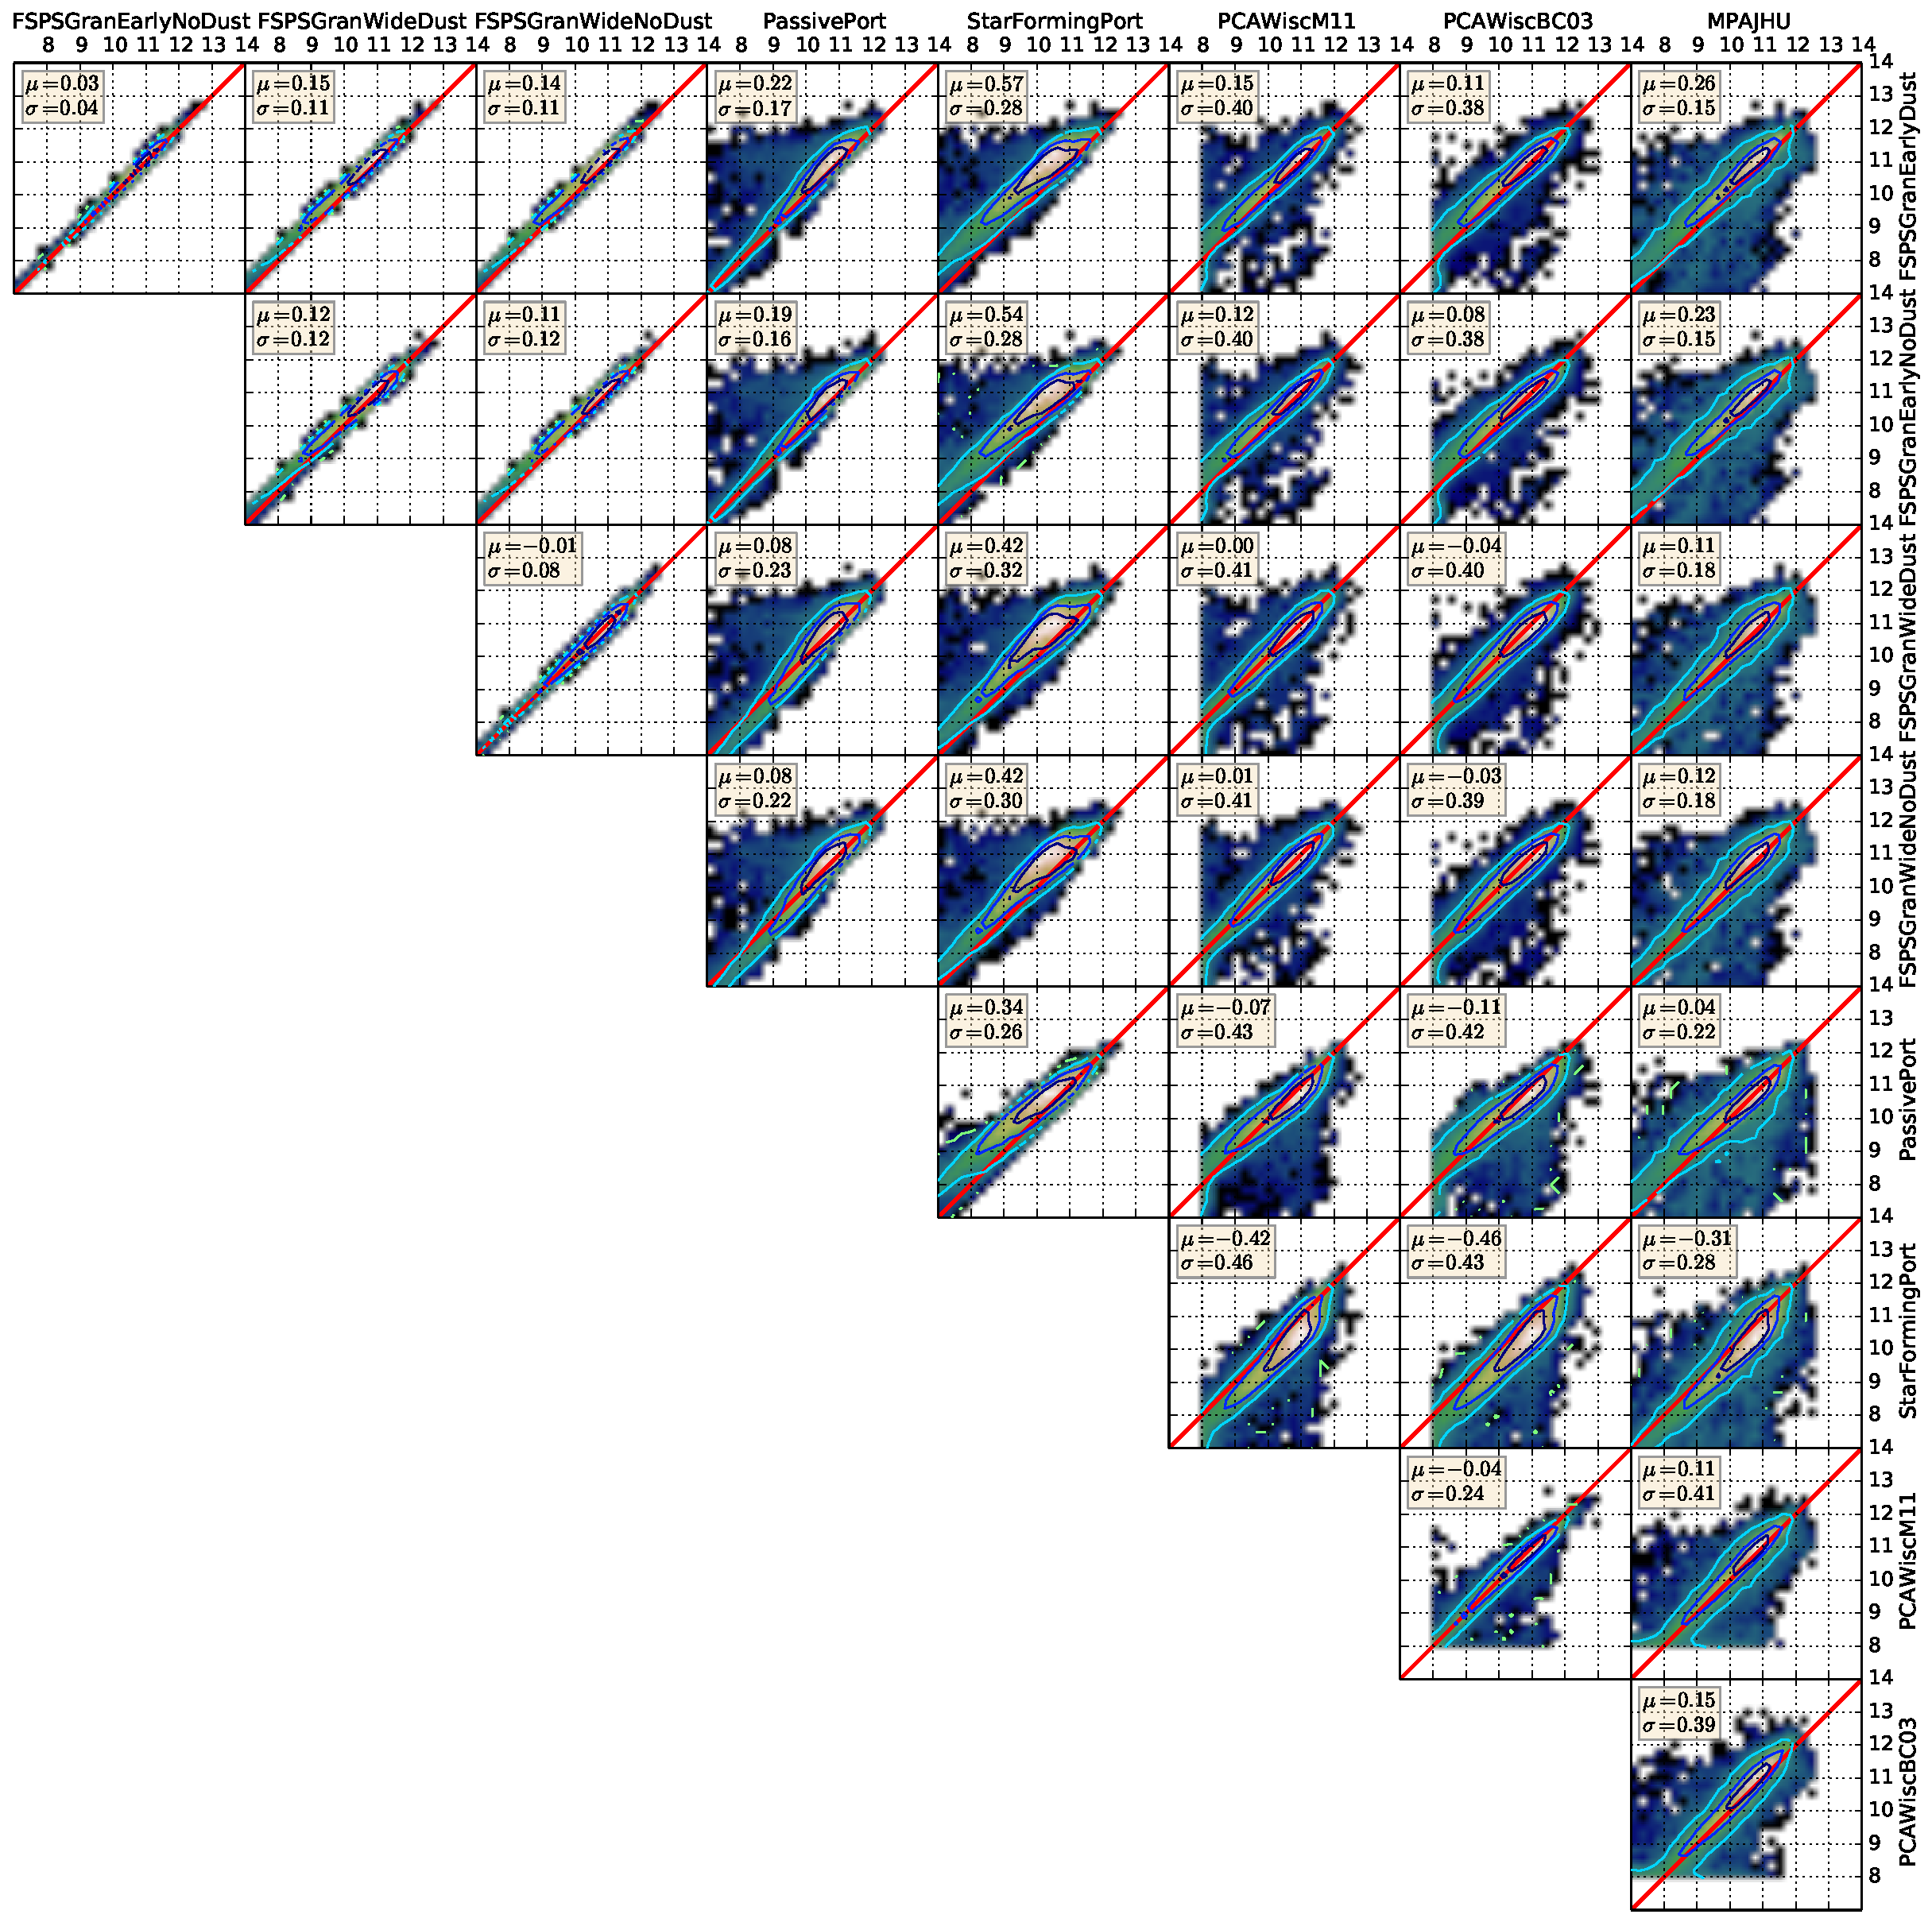
\includegraphics[width=\linewidth]{stellar_mass_models.pdf}
                % }
                % \only<4>{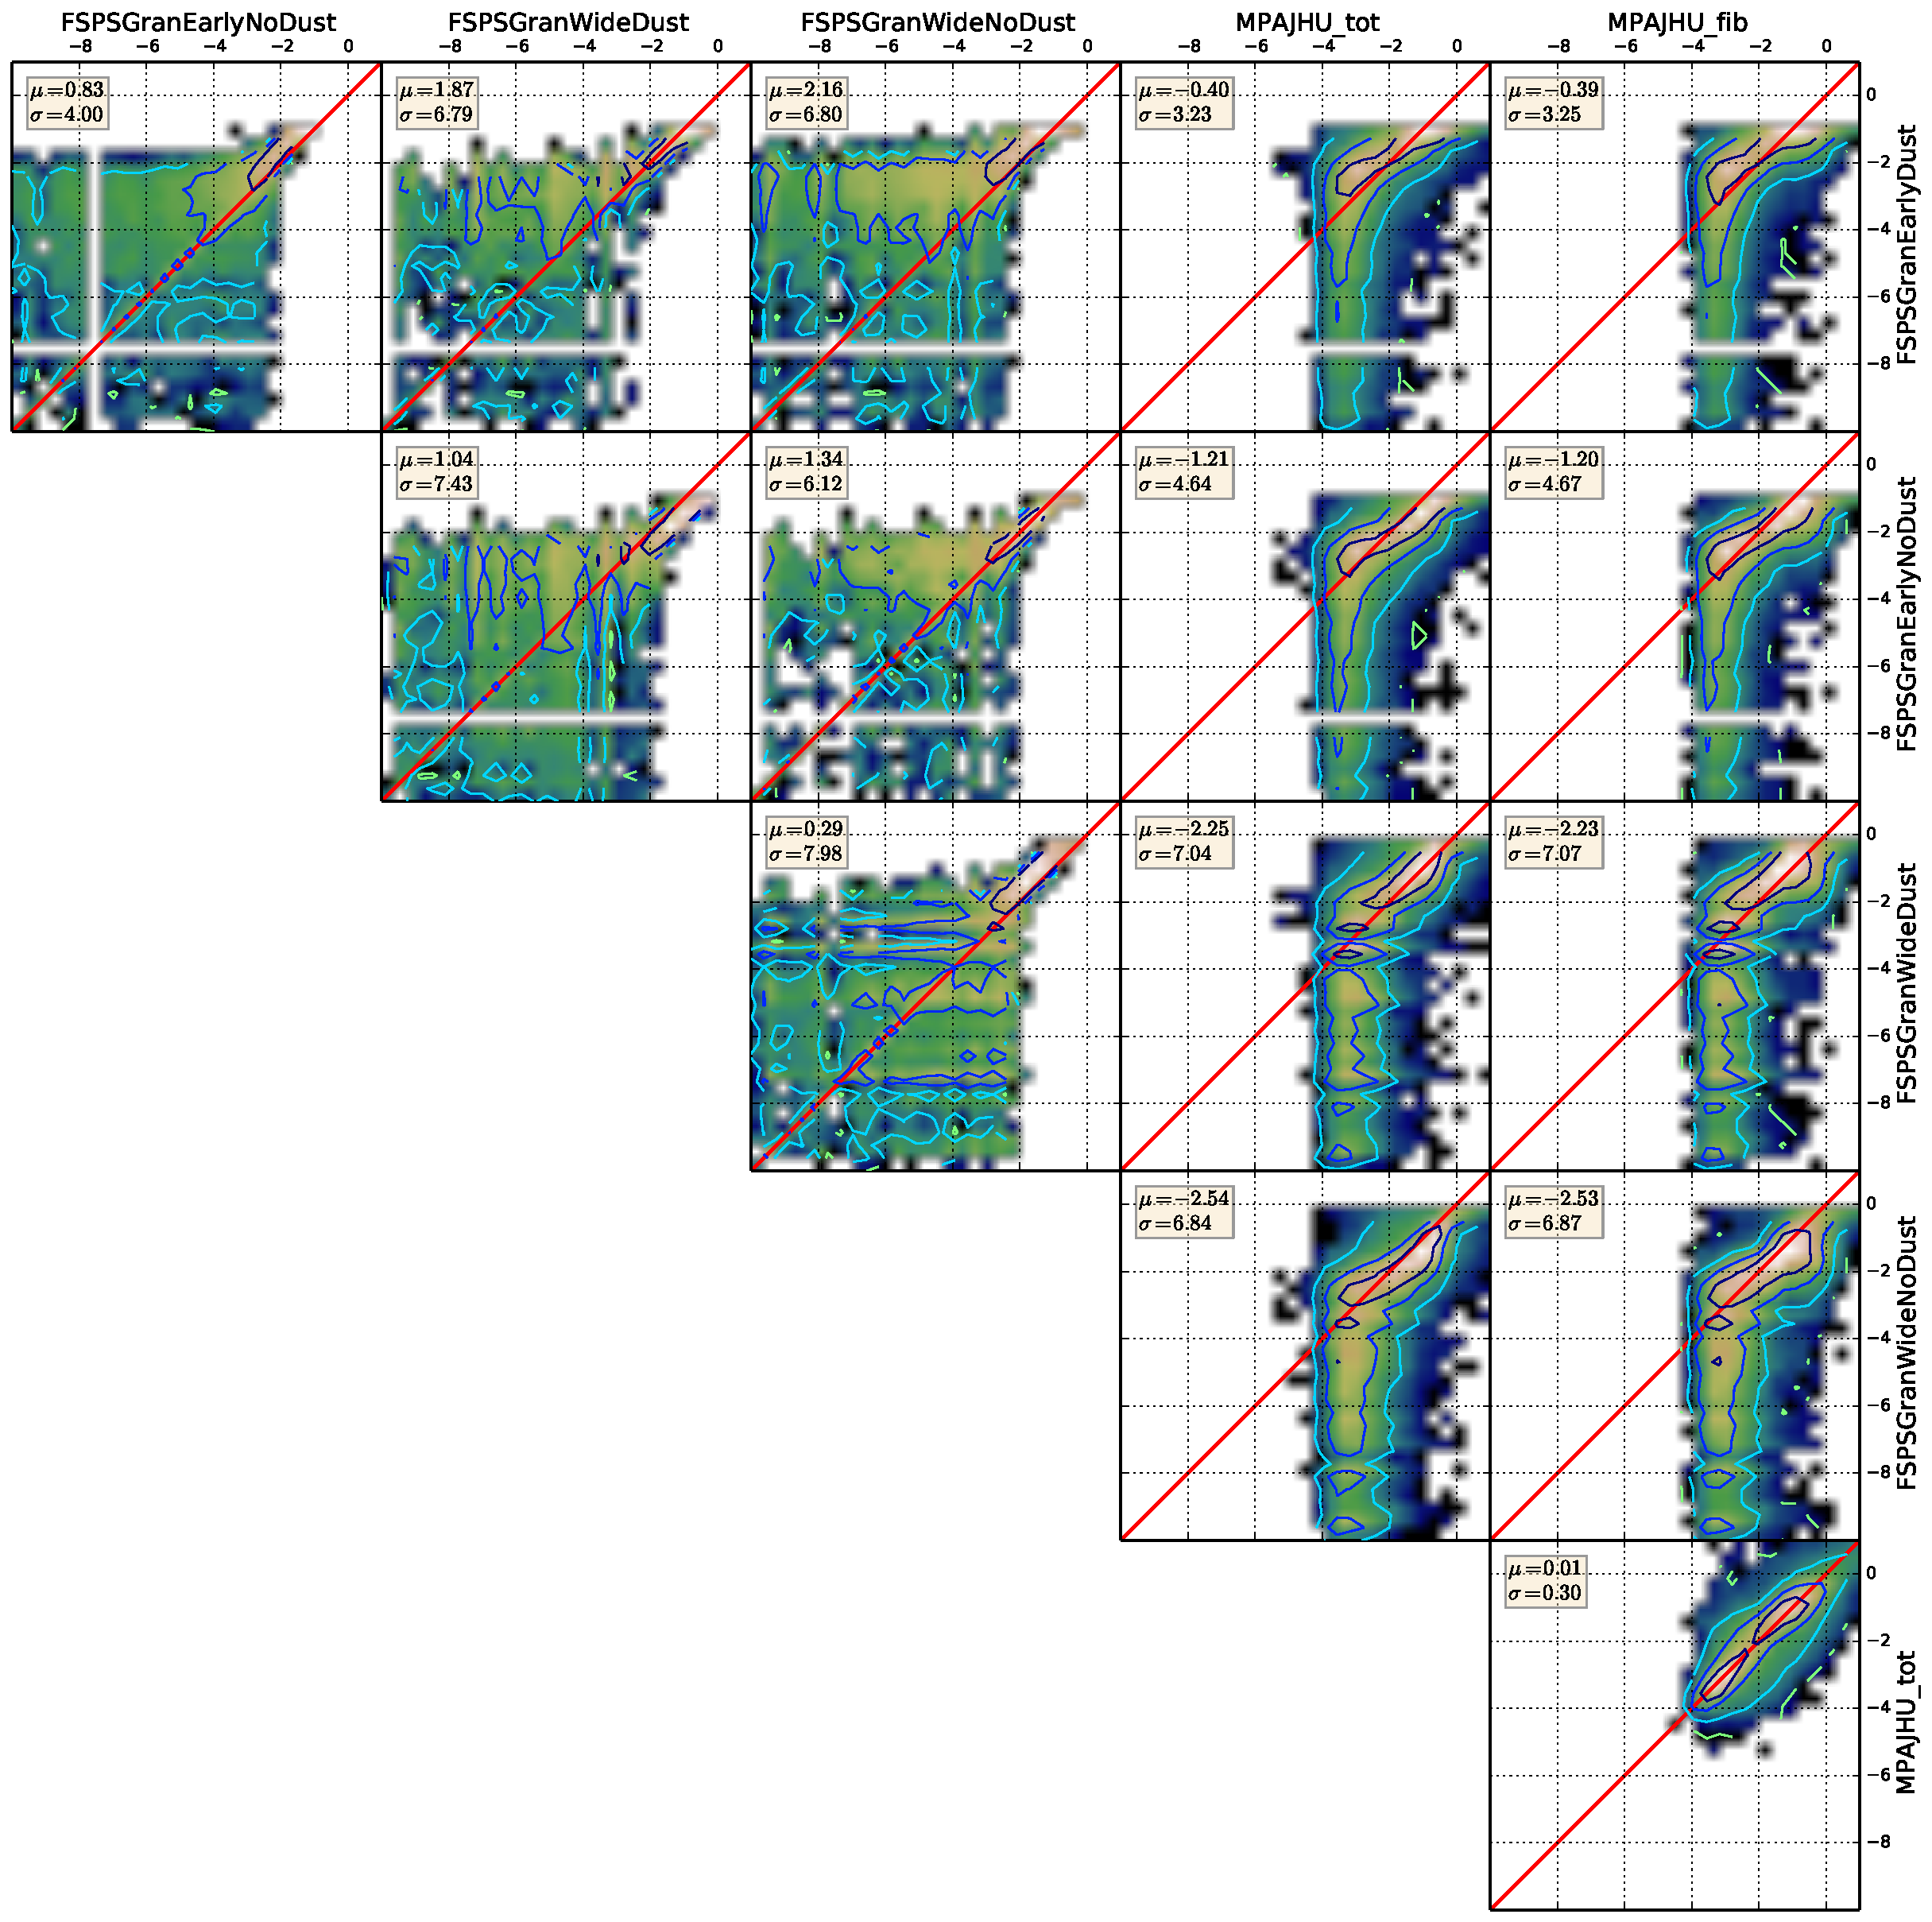
\includegraphics[width=\linewidth]{ssfr_models.pdf}}
            % \end{minipage}
        % \end{column}
        % \begin{column}{0.4\linewidth}
            \begin{minipage}[c][0.7\textheight][c]{\linewidth}
                \begin{block}{Difficulties}
                    \begin{itemize}
                        \item<1-> Clean galaxy sample without bad photometry,
                            false detection, etc
                        \item<2-> Handle bright stars, holes, etc
                        \item<3-> Stellar masses and SSFR estimations
                        \item<4-> We use the galaxy sample of \citet{Tempel+14}
                    \end{itemize}
                \end{block}
            \end{minipage}
        % \end{column}
    % \end{columns}
\end{frame}

\subsection{Environmental effects}
\begin{frame}
    \frametitle{Application to SDSS}

    \begin{columns}
        \begin{column}{0.59\linewidth}
            \centering
            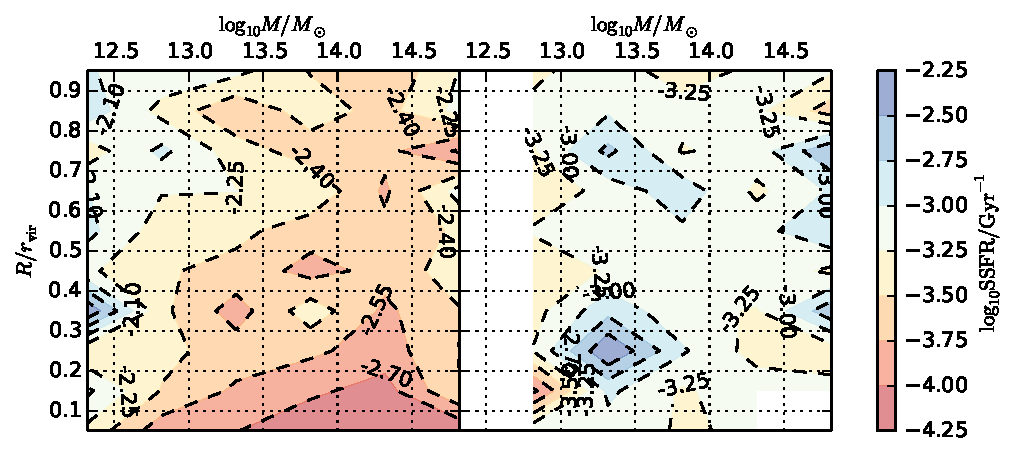
\includegraphics[width=\linewidth]{mean_ssfr.pdf}\\
            Mean $\log_{10}$ SSFR
        \end{column}
        \begin{column}{0.59\linewidth}
            \centering
            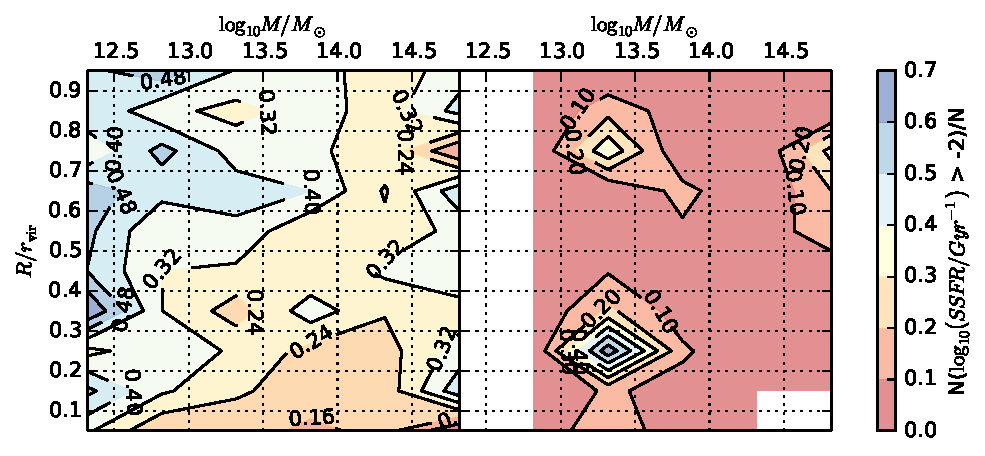
\includegraphics[width=\linewidth]{young.pdf}\\
            Fraction of active galaxies
        \end{column}
    \end{columns}
    \begin{block}{Preliminary results}
        \begin{enumerate}
            \item<1-> Poor statistics
            \item<2-> Trends depend on MAGGIE or FoF group finder
        \end{enumerate}
    \end{block}
\end{frame}
